\documentclass[11pt]{amsart}
\pdfsuppressptexinfo=-1
\usepackage[T1]{fontenc}
\usepackage{lmodern}
\usepackage[margin=1.1in]{geometry}
\usepackage{amsmath,amssymb,amsthm,mathtools}
\usepackage{enumitem}
\usepackage{tikz}
\usepackage[hidelinks]{hyperref}
\hypersetup{pdftitle={An upper bound of 2√2 for the three-dimensional sofa problem in a snake-shaped corridor},
  pdfauthor={Tejasvi Singh Tomar}}

\newtheorem{theorem}{Theorem}[section]
\newtheorem{lemma}[theorem]{Lemma}
\newtheorem{proposition}[theorem]{Proposition}
\newtheorem{corollary}[theorem]{Corollary}
\theoremstyle{definition}
\newtheorem{definition}[theorem]{Definition}
\theoremstyle{remark}
\newtheorem{remark}[theorem]{Remark}
\numberwithin{equation}{section}
\setlength{\emergencystretch}{2em}
\raggedbottom

\newcommand{\R}{\mathbb{R}}
\newcommand{\vol}{\operatorname{vol}}
\newcommand{\area}{\operatorname{area}}
\newcommand{\one}{\mathbf{1}}
% Release slots (fixed at the freeze).
\newcommand{\ZENODODOI}{10.5281/zenodo.23716060}
\newcommand{\REPOURL}{https://github.com/tejasvi/snake-sofa-bound/tree/v3}

\begin{document}

\title[The sofa problem in a snake-shaped corridor]{An upper bound of $2\sqrt{2}$ for the three-dimensional sofa problem in a snake-shaped corridor}
\author{Tejasvi Singh Tomar}
\renewcommand{\urladdrname}{{\itshape ORCID}}
\urladdr{\href{https://orcid.org/0000-0003-4668-3639}{https://orcid.org/0000-0003-4668-3639}}
\subjclass[2020]{51M16, 49Q10; 52A38, 68V20}
\keywords{Moving sofa problem, snake-shaped corridor, rigid motion, intersection of tubes, volume bound, formal verification}

\begin{abstract}
The moving sofa problem in a snake-shaped corridor, posed by O'Rourke and by Georgiev, G\'omez-Serrano, Tao and Wagner, asks for the largest volume of a connected body that can be moved through a corridor of unit-square cross-section with two turns that are far apart, one in the $x$--$y$ plane and one in the $y$--$z$ plane. The largest reported body has volume at least $1.8558404$, and Tang obtained upper bounds for this problem, the best of which is $3.4083$. We prove by hand that the largest volume is at most $2\sqrt2$ whenever the straight section between the turns is longer than $2+\sqrt2$. The main new tool is a sharp bound: two infinite tubes of unit-square cross-section whose axes make an angle~$\theta$ meet in volume at most $1/\sin\theta$. With it, Hammersley's argument for the planar moving sofa problem carries over to three dimensions. The same argument gives explicit bounds for shorter straight sections; these and the main bound have also been proved in Lean~4 with Mathlib.
\end{abstract}

\maketitle

\section{Introduction}\label{sec:intro}

The moving sofa problem, posed by Moser in 1966 \cite{Mos66}, asks for the largest area of a connected planar region that can be moved around a right-angled corner in a hallway of unit width. Two years later Hammersley \cite{Ham68} proved that the area is at most $2\sqrt2$. In 1992 Gerver \cite{Ger92} constructed a region of area $2.2195\ldots$; Kallus and Romik \cite{KR18} later lowered the upper bound to $2.37$ with the help of a computer, and Baek \cite{Bae24} has given a proof that Gerver's region is optimal. Romik \cite{Rom18} extended Gerver's method and found, in closed form, a candidate for the variant in which the region must turn both ways.

In 2016 O'Rourke \cite{ORo16} posed a three-dimensional version. A corridor of unit-square cross-section has an entry arm parallel to the $x$-axis, a middle arm parallel to the $y$-axis and an exit arm parallel to the $z$-axis. The first turn lies in the $x$--$y$ plane and the second in the $y$--$z$ plane. Georgiev, G\'omez-Serrano, Tao and Wagner \cite[Problem~6.64]{GGTW25} ask for the largest volume $C_{6.64}$ of a connected bounded set that can pass continuously through such a corridor when the two turns are far apart. The code that accompanies \cite{GGTW25} uses a straight section of length $4$ between the turns \cite[Definition~2.1]{Tan26a}. The authors of \cite{GGTW25} report a body of volume at least $1.81$. Tang \cite{Tan26b} reports one of volume at least $1.8558404$, certified with the same code. Tang \cite{Tan26a} also proved upper bounds: for a straight section of length $M$, the bound $4.2862$ for $M\ge2.61$ is proved by hand, while the best bound, $3.4083$ for $M>2.2$, rests on a branch-and-bound computation in double precision.

We define the corridor $K_M$ and passages in Section~\ref{sec:setup} and write $V^*(K_M)$ for the supremum of the volumes of compact connected sets that pass through $K_M$.

\begin{theorem}\label{thm:main}
For every $M>2+\sqrt2$, we have $V^*(K_M)\le 2\sqrt2$.
\end{theorem}

The bound $2\sqrt2=2.8284\ldots$ does not depend on $M$. It therefore holds for each reading of ``far apart'' with $M>2+\sqrt2$, including $M=4$. In the notation of \cite{GGTW25}, where the bodies are bounded connected sets, it gives $C_{6.64}\le2\sqrt2$ by Remark~\ref{rem:readings}, which also treats other readings of the problem. Since the proof does not use the second turn, the bound also holds for a corridor with one turn (Corollary~\ref{cor:oneturn}).

\subsection*{The method}
The body starts in the entry arm, so at each time it lies in a moving copy of the infinite tube $\R\times[0,1]^2$, which we call its \emph{entry tube}. Our proof adds two steps to the first-crossing argument of Tang \cite{Tan26a}. First, we prove that two infinite tubes of unit-square cross-section whose axes make an angle $\theta$ meet in volume at most $1/\sin\theta$ (Lemma~\ref{lem:twotube}). This bound, sharp for every $\theta$, is the bound conjectured in \cite[Remark~8.1]{Tan26a}. Second, we combine it with Tang's argument, which looks at the first time at which the body reaches a given height in the middle arm. We take the plane $y=3+\sqrt2$; this plane must cut the straight section, which is why Theorem~\ref{thm:main} assumes $M>2+\sqrt2$. Unless the volume is less than $\sqrt2$, the axis of the entry tube makes the angle $\pi/4$ with the middle arm, and hence, since the arms are perpendicular, an angle of at least $\pi/4$ with the entry arm, at some time up to that first time (Section~\ref{sec:proof}). The body then lies in the union of the entry arm and the middle arm, where Lemma~\ref{lem:twotube} bounds the parts of the body in the two arms by $\sqrt2$ each.

This is Hammersley's argument in three dimensions: in the plane, after a rotation by $\pi/4$ the sofa lies in a strip of width one that makes the angle $\pi/4$ with both arms of the hallway, and this strip meets each arm in area at most $\sqrt2$ \cite[Section~2]{KR18}; Figure~\ref{fig:strip} shows the corresponding position in three dimensions. Section~\ref{sec:limits} shows that, in three dimensions as in the plane, the information used at this one time cannot give a bound below $2\sqrt2$: a tube whose axis makes the angle $\pi/4$ with the middle arm can meet the first two arms in volume exactly $2\sqrt2$ (Proposition~\ref{prop:relax}). A smaller bound needs more information, such as the positions of the body at several times, which Kallus and Romik combine in the plane \cite{KR18}.

\begin{figure}[ht]
\centering
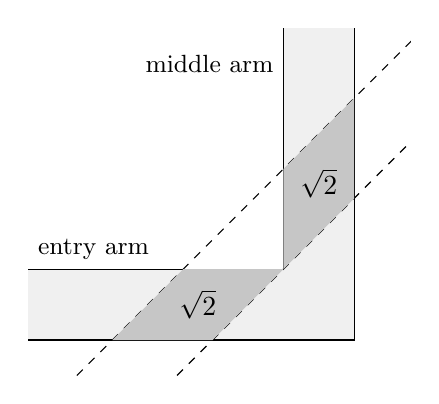
\begin{tikzpicture}[scale=0.9]
\fill[gray!12] (-3.6,0)--(1,0)--(1,4.4)--(0,4.4)--(0,1)--(-3.6,1)--cycle;
\draw (-3.6,0)--(1,0)--(1,4.4) (0,4.4)--(0,1)--(-3.6,1);
\begin{scope}
\clip (-3.6,-0.5) rectangle (1.8,4.4);
\draw[dashed] (-1.5,-0.5)--(3.4,4.4);
\draw[dashed] (-2.9142,-0.5)--(1.9858,4.4);
\end{scope}
\fill[gray!45] (-2.4142,0)--(-1,0)--(0,1)--(-1.4142,1)--cycle;
\fill[gray!45] (0,1)--(1,2)--(1,3.4142)--(0,2.4142)--cycle;
\node at (-1.2071,0.5) {$\sqrt2$};
\node at (0.5,2.2071) {$\sqrt2$};
\node[above right] at (-3.6,1) {\small entry arm};
\node[left] at (0,3.9) {\small middle arm};
\end{tikzpicture}
\caption{The cross-section $z=\mathrm{const}$, $0\le z\le1$, of the first two arms of the corridor (light) and of the tube of Proposition~\ref{prop:relax} whose axis makes the angle $\pi/4$ with both arms (between the dashed lines). The tube meets each arm in a parallelogram of area $\sqrt2$ (dark), and so in volume $\sqrt2$.}\label{fig:strip}
\end{figure}

Section~\ref{sec:more} applies the same argument to shorter straight sections; together with Theorem~\ref{thm:main}, the resulting bounds improve those of \cite{Tan26a} for every $M>\sqrt2$ outside the interval $(2.2,2.26)$ (Table~\ref{tab:compare}). Section~\ref{sec:open} states the open questions, and Appendix~\ref{sec:lean} describes a formalization of the main results in Lean~4 with Mathlib.

\section{The corridor and passages}\label{sec:setup}

We write $e_x,e_y,e_z$ for the standard basis of $\R^3$ and $\vol$ for Lebesgue measure. For $c\in\R$ we write $\{y\le c\}$ for the half-space $\{p\in\R^3:p\cdot e_y\le c\}$, and similarly for other inequalities.

\begin{definition}\label{def:corridor}
Let $M>0$. The \emph{corridor} is $K_M=S_X\cup S_Y\cup S_Z$, where
\[
S_X=(-\infty,0]\times[0,1]\times[0,1],\quad S_Y=[0,1]\times[0,1+M]\times[0,1],\quad S_Z=[0,1]\times[1+M,2+M]\times[0,\infty).
\]
\end{definition}

The cube $[0,1]^3$ is the first corner, where the corridor turns from the $x$-direction into the $y$-direction. The cube $[0,1]\times[1+M,2+M]\times[0,1]$ is the second corner, where it turns into the $z$-direction. Between the corners lies a straight section of length $M$. These are the corridors of \cite[Definition~2.1]{Tan26a}. Other choices of the directions of the turns give images of $K_M$ under reflections, which preserve volumes and passages.

For $c\ge0$ we put
\[
S_Y(c)=[0,1]\times[0,c]\times[0,1],\qquad W_c=[0,1]\times\{c\}\times[0,1].
\]
We also use the infinite tubes $X=\R\times[0,1]\times[0,1]$ and $Y=[0,1]\times\R\times[0,1]$. Since $S_X\subseteq\{y\le1\}$, $S_Y\cap\{y\le c\}=S_Y(c)$ and $S_Z\subseteq\{y\ge1+M\}$, we have
\begin{equation}\label{eq:low}
K_M\cap\{y\le c\}=S_X\cup S_Y(c)\subseteq X\cup Y\qquad(1\le c<1+M).
\end{equation}
In particular, $K_M\cap\{y\le1\}=(-\infty,1]\times[0,1]\times[0,1]\subseteq X$.

A \emph{rigid motion} is a map $g(p)=Rp+v$ with $R\in SO(3)$ and $v\in\R^3$. The rigid motions form the group $SE(3)$, which we view as a subset of $\R^{3\times3}\times\R^3$.

\begin{definition}\label{def:passage}
A \emph{body} is a nonempty compact connected set $B\subset\R^3$. A \emph{passage} of $B$ through $K_M$ is a continuous map $t\mapsto g_t$ from $[0,1]$ to $SE(3)$ such that the sets $B_t=g_t(B)$ satisfy
\begin{enumerate}[label=(\roman*)]
\item\label{p:in} $B_t\subseteq K_M$ for all $t\in[0,1]$,
\item\label{p:start} $B_0\subseteq S_X$,
\item\label{p:end} $B_1\subseteq S_Z$.
\end{enumerate}
We write $V^*(K_M)$ for the supremum of $\vol(B)$ over all bodies $B$ that have a passage through $K_M$.
\end{definition}

This is the weak traversal of \cite[Definition~2.2]{Tan26a}. There a body must also have positive volume, which does not change $V^*(K_M)$.

\begin{remark}[Other readings]\label{rem:readings}
The proof of Theorem~\ref{thm:main} uses the conditions \ref{p:start} and \ref{p:end} only in the weaker forms
\begin{enumerate}[label=(\roman*$'$)]
\setcounter{enumi}{1}
\item\label{p:start2} $B_0\subseteq K_M\cap\{y\le1\}$,
\item\label{p:end2} $B_1$ meets $\{y\ge1+M\}$.
\end{enumerate}
The theorem therefore holds for each notion of passage that implies \ref{p:in}, \ref{p:start2} and \ref{p:end2}. Stronger conditions on the end positions, such as $B_1\subseteq S_Z\cap\{z\ge1\}$ or the fixed start and end positions in the code of \cite{GGTW25} (see \cite[Remark~2.3]{Tan26a}), are of this kind. If a bounded connected set $E$ passes, then its closure is a body that passes with the same motion, because $K_M$, $S_X$ and $S_Z$ are closed. Its volume is at least the outer measure of $E$. Similarly, if $E$ passes through the interior of $K_M$, with the interiors of $S_X$ and $S_Z$ as start and end regions, then its closure passes through $K_M$.
\end{remark}

\section{Two tubes}\label{sec:tubes}

We first bound the volume of the intersection of two tubes with unit-square cross-sections.

\begin{definition}\label{def:tube}
A \emph{tube} is a set
\[
T=\bigl\{\rho+\lambda e+af_1+bf_2:\ \lambda\in\R,\ |a|\le\tfrac12,\ |b|\le\tfrac12\bigr\},
\]
where $(e,f_1,f_2)$ is an orthonormal basis of $\R^3$ and $\rho\in\R^3$. The line $\rho+\R e$ is the \emph{axis} of $T$, the vector $e$ is an \emph{axis direction}, and the unit square $Q=\{af_1+bf_2:|a|,|b|\le\frac12\}$ in the plane $e^\perp$ is the \emph{cross-section}. The \emph{angle} between two tubes with axis directions $e$ and $e'$ is the angle $\theta\in[0,\pi/2]$ between their axes, so that $\cos\theta=|e\cdot e'|$.
\end{definition}

Each $p\in\R^3$ can be written uniquely as $p=\rho+\lambda e+\xi$ with $\lambda\in\R$ and $\xi\in e^\perp$. In this decomposition, $p\in T$ if and only if $\xi\in Q$; here $\rho$ lies on the axis and $Q$ is centred at $0$. Rigid motions map tubes to tubes. The sets $X$ and $Y$ are tubes with axis directions $e_x$ and $e_y$.

\begin{lemma}\label{lem:chord}
Let $Q$ be a unit square centred at $0$ in a plane, and let $m,n$ be orthonormal vectors in this plane. For $b\in\R$ let $\ell(b)$ be the length of the interval $\{a\in\R:am+bn\in Q\}$. Then $\int_\R\ell(b)^2\,db\le1$, with equality if and only if $m$ is parallel to a side of $Q$.
\end{lemma}

\begin{proof}
Let $\gamma(x)=\area(Q\cap(Q+x))$ for $x$ in the plane. For $\xi=am+bn$, the set of $r\in\R$ with $\xi-rm\in Q$ is an interval of length $\ell(b)$. By Tonelli's theorem,
\[
\int_\R\gamma(rm)\,dr=\int_\R\int\one_Q(\xi)\,\one_Q(\xi-rm)\,d\xi\,dr=\int\one_Q(\xi)\,\ell(\xi\cdot n)\,d\xi=\int_\R\ell(b)^2\,db.
\]
Let $d_1,d_2$ be unit vectors along the sides of $Q$, and let $\kappa\ge\sigma\ge0$ be the numbers $|m\cdot d_1|$ and $|m\cdot d_2|$ in decreasing order. Then $\kappa^2+\sigma^2=1$, so $\kappa\ge1/\sqrt2$. Since $\gamma(x)=(1-|x\cdot d_1|)_+(1-|x\cdot d_2|)_+$, and since $1-r\sigma\ge1-\sigma/\kappa\ge0$ for $0\le r\le1/\kappa$, we get
\[
\int_\R\gamma(rm)\,dr=2\int_0^{1/\kappa}(1-r\kappa)(1-r\sigma)\,dr=\frac1\kappa-\frac{\sigma}{3\kappa^2}.
\]
This is at most $1$ if and only if $3\kappa(1-\kappa)\le\sigma$. If $\sigma=0$, then $\kappa=1$ and equality holds. If $\sigma>0$, then $1-\kappa=\sigma^2/(1+\kappa)$, so the inequality becomes $3\kappa\sigma\le1+\kappa$. It holds strictly, because $3\kappa\sigma\le\frac32(\kappa^2+\sigma^2)=\frac32<1+\frac1{\sqrt2}\le1+\kappa$.
\end{proof}

\begin{lemma}\label{lem:twotube}
Let $T$ and $T'$ be tubes at angle $\theta\in(0,\pi/2]$. Then
\[
\vol(T\cap T')\le\frac1{\sin\theta}.
\]
Equality holds if and only if both tubes have a pair of faces orthogonal to the unit normal $n$ of the plane spanned by their axis directions, and $T$ and $T'$ have the same orthogonal projection to the line $\R n$.
\end{lemma}

\begin{proof}
Write $T=\{\rho+\lambda e+\xi:\lambda\in\R,\ \xi\in Q\}$ and $T'=\{\rho'+\lambda e'+\xi:\lambda\in\R,\ \xi\in Q'\}$ as in Definition~\ref{def:tube}. Let $n=e\times e'/|e\times e'|$, where $|e\times e'|=\sin\theta>0$, and put $m=n\times e$ and $m'=n\times e'$. Then $(e,m,n)$ and $(e',m',n)$ are orthonormal bases, and $m\cdot m'=e\cdot e'$. Let $\ell$ and $\ell'$ be the functions of Lemma~\ref{lem:chord} for $Q$ with $(m,n)$ and for $Q'$ with $(m',n)$.

We slice by the planes $P_g=\{p:p\cdot n=g\}$, $g\in\R$. A point $p\in P_g$ has the form $\rho+\lambda e+am+bn$ with $b=g-\rho\cdot n$, so $p\in T$ if and only if $(p-\rho)\cdot m$ lies in an interval of length $\ell(g-\rho\cdot n)$. Similarly, $p\in T'$ if and only if $(p-\rho')\cdot m'$ lies in an interval of length $\ell'(g-\rho'\cdot n)$. Since the unit vectors $m$ and $m'$ lie in the plane $n^\perp$ and $|m\cdot m'|=\cos\theta$, the map $p\mapsto(p\cdot m,p\cdot m')$ from $P_g$ to $\R^2$ is affine with Jacobian $\sin\theta$, and
\[
\area(T\cap T'\cap P_g)=\frac{\ell(g-\rho\cdot n)\,\ell'(g-\rho'\cdot n)}{\sin\theta}.
\]
We integrate over $g$ and apply the Cauchy--Schwarz inequality and Lemma~\ref{lem:chord}:
\[
\vol(T\cap T')=\frac1{\sin\theta}\int_\R\ell(g-\rho\cdot n)\,\ell'(g-\rho'\cdot n)\,dg\le\frac1{\sin\theta}\Bigl(\int_\R\ell^2\Bigr)^{1/2}\Bigl(\int_\R\ell'^2\Bigr)^{1/2}\le\frac1{\sin\theta}.
\]
If equality holds, then $\int\ell^2=\int\ell'^2=1$, since both integrals are at most $1$ and the product of their square roots is $1$. Lemma~\ref{lem:chord} then shows that $m$ is parallel to a side of $Q$. Then $n$ is parallel to the other side, so $T$ has a pair of faces orthogonal to $n$, and $\ell$ is the indicator function of $[-\frac12,\frac12]$. The same holds for $T'$. Equality in the Cauchy--Schwarz inequality then forces $\rho\cdot n=\rho'\cdot n$. Conversely, under these conditions the integral equals $\int_\R\one_{[-1/2,1/2]}(g-\rho\cdot n)\,dg=1$.
\end{proof}

\begin{remark}\label{rem:twotube}
Tang \cite[Lemma~7.1]{Tan26a} proves the bound $\sqrt2/\sin\theta$. Equality holds in Lemma~\ref{lem:twotube}, for example, for $X$ and the tube $\{p:|p\cdot(-\sin\theta,\cos\theta,0)|\le\frac12,\ 0\le p\cdot e_z\le1\}$. Their intersection is the product of a parallelogram of area $1/\sin\theta$ with $[0,1]$.
\end{remark}

\section{Proof of the main theorem}\label{sec:proof}

In this section we fix $M>0$, a body $B$, and a continuous map $t\mapsto g_t$ from $[0,1]$ to $SE(3)$ that satisfies \ref{p:in}, \ref{p:start2} and \ref{p:end2}. We write $g_t(p)=R_tp+v_t$ and $B_t=g_t(B)$. Replacing $B$ by $B_0$ and $g_t$ by $g_tg_0^{-1}$ changes neither the sets $B_t$ nor the volume, since $\vol(B_0)=\vol(B)$, so we may assume that $g_0$ is the identity. We include short proofs of Lemmas~\ref{lem:entry}--\ref{lem:tilt}, which are due to Tang \cite{Tan26a}.

\subsection{The entry tube and the height}

\begin{lemma}[{\cite[Lemmas~3.2 and~3.3]{Tan26a}}]\label{lem:entry}
\begin{enumerate}[label=(\alph*)]
\item For each $t\in[0,1]$, the set $B_t$ lies in the tube $T_t=g_t(X)$, whose axis direction is $w_t=R_te_x$. The function $\mu(t)=|w_t\cdot e_y|$ is continuous on $[0,1]$, with $\mu(0)=0$.
\item The function $h(t)=\max\{p\cdot e_y:p\in B_t\}$ is continuous on $[0,1]$, with $h(0)\le1$ and $h(1)\ge1+M$.
\end{enumerate}
\end{lemma}

\begin{proof}
(a) By \ref{p:start2}, $B=B_0\subseteq K_M\cap\{y\le1\}\subseteq X$. Hence $B_t=g_t(B)\subseteq g_t(X)$. The rotation part $R_t$ of $g_t$ maps the axis direction $e_x$ of $X$ to $w_t$. The map $t\mapsto w_t$ is continuous, with $w_0=e_x$ because $R_0$ is the identity.

(b) For $p\in B$ and $t,t'\in[0,1]$ we have $|g_t(p)-g_{t'}(p)|\le\|R_t-R_{t'}\|\max_{q\in B}|q|+|v_t-v_{t'}|$, with the operator norm. The right side does not depend on $p$ and tends to $0$ as $t'\to t$, so $|h(t)-h(t')|$ tends to $0$. Finally, $h(0)\le1$ by \ref{p:start2} and $h(1)\ge1+M$ by \ref{p:end2}.
\end{proof}

\subsection{The first crossing}

\begin{lemma}[{\cite[Lemmas~3.4 and~3.5]{Tan26a}}]\label{lem:event}
Let $1<c<1+M$, and let $\tau=\min\{t\in[0,1]:h(t)\ge c\}$.
\begin{enumerate}[label=(\alph*)]
\item The minimum exists, and $B_t\subseteq S_X\cup S_Y(c)$ for all $t\in[0,\tau]$.
\item The set $B_\tau$ contains a point of $W_c$.
\item If $B_\tau$ meets $\{y\le1\}$, then $B_\tau$ contains a point of $W_1$.
\end{enumerate}
\end{lemma}

\begin{proof}
(a) By Lemma~\ref{lem:entry}(b), the set $\{t:h(t)\ge c\}$ is closed and contains $1$, so $\tau$ exists. Since $h(0)\le1<c$, we have $\tau>0$ and $h(t)<c$ for $t<\tau$; by continuity, $h(\tau)=c$. Hence $B_t\subseteq K_M\cap\{y\le c\}$ for $t\le\tau$, which gives (a) by \eqref{eq:low}.

(b) Since $B_\tau$ is compact, some $q\in B_\tau$ has $q\cdot e_y=h(\tau)=c>1$. By (a) and $S_X\subseteq\{y\le1\}$, we have $q\in S_Y(c)$, so $q\in W_c$.

(c) The sets $A_1=B_\tau\cap\{y\le1\}$ and $A_2=B_\tau\cap\{y>1\}$ are disjoint and nonempty, their union is $B_\tau$, and $A_1$ is closed. Since $B_\tau$ is connected, $A_2$ is not closed, so some point $p\in B_\tau\setminus A_2$ is a limit of points of $A_2$. Then $p\cdot e_y=1$. By (a), the points of $A_2$ lie in $S_Y(c)$, so their $x$- and $z$-coordinates lie in $[0,1]$, and so do those of $p$. Thus $p\in W_1$.
\end{proof}

\subsection{The tilt}

\begin{lemma}[{\cite[Lemma~5.1]{Tan26a}}]\label{lem:tilt}
Let $u>\sqrt2$ and $\mu^*(u)=(u^2-2)/(u^2+2)$. If a tube with axis direction $w$ contains a point $p\in W_1$ and a point $q\in W_{1+u}$, then $|w\cdot e_y|\ge\mu^*(u)$.
\end{lemma}

\begin{proof}
Let $\mu=|w\cdot e_y|$ and $\nu=\sqrt{1-\mu^2}$. Write $d=q-p=(d_x,u,d_z)$ and $r=(d_x^2+d_z^2)^{1/2}$. Then $r\le\sqrt2$, because $p$ and $q$ have $x$- and $z$-coordinates in $[0,1]$. Write the tube as $\{\rho+\lambda w+\xi:\lambda\in\R,\ \xi\in Q\}$. The component $d-(d\cdot w)w$ of $d$ orthogonal to $w$ is the difference of two points of $Q$, a square of diameter $\sqrt2$. Hence $|d|^2-(d\cdot w)^2\le2$. By the Cauchy--Schwarz inequality, $|d\cdot w|\le u\mu+|d_xw_x+d_zw_z|\le u\mu+r\nu$. Since $|d|^2=u^2+r^2$, we get
\[
u^2+r^2-2\le(u\mu+r\nu)^2.
\]
Since $\mu^2+\nu^2=1$, this is equivalent to $(u\nu-r\mu)^2\le2$, and therefore $u\nu\le\sqrt2+r\mu\le\sqrt2\,(1+\mu)$. As $\nu=\sqrt{1-\mu}\sqrt{1+\mu}$ and $1+\mu>0$, we get $u\sqrt{1-\mu}\le\sqrt2\sqrt{1+\mu}$. Squaring gives $u^2(1-\mu)\le2(1+\mu)$, that is, $\mu\ge\mu^*(u)$.
\end{proof}

\begin{remark}\label{rem:tilt}
Lemma~\ref{lem:tilt} is sharp. Let $p=(0,1,0)$, $q=(1,1+u,1)$ and $w=(\nu/\sqrt2,\mu^*(u),\nu/\sqrt2)$ with $\nu=\sqrt{1-\mu^*(u)^2}$. A short computation shows that $|q-p|^2-((q-p)\cdot w)^2=2$, that is, the component of $q-p$ orthogonal to $w$ has length $\sqrt2$. Therefore $p$ and $q$ lie in a tube with axis direction $w$ whose cross-section has this component as a diagonal.
\end{remark}

\subsection{The volume bound}

\begin{proposition}\label{prop:pose}
Let $\sqrt2<u<M$ and $0<s\le\mu^*(u)$. Then
\[
\vol(B)\le\frac1s+\frac1{\sqrt{1-s^2}}.
\]
\end{proposition}

\begin{proof}
Put $c=1+u$, so that $1<c<1+M$, and let $\tau$ be as in Lemma~\ref{lem:event}. Since $\mu^*(u)<1$, we have $s<1$. We first show that $\vol(B)<1/\sqrt{1-s^2}$ or $\mu(\tau)\ge s$.

Suppose that $B_\tau\subseteq\{y>1\}$. By Lemma~\ref{lem:event}(a), and since $S_X$ lies in $\{y\le1\}$, we have $B_\tau\subseteq S_Y(c)\subseteq Y$. Also $B_\tau\subseteq T_\tau$ by Lemma~\ref{lem:entry}(a). If $\mu(\tau)<s$, then the angle $\theta$ between $T_\tau$ and $Y$ satisfies $\cos\theta=\mu(\tau)<s$, so Lemma~\ref{lem:twotube} gives
\[
\vol(B)=\vol(B_\tau)\le\vol(T_\tau\cap Y)\le\frac1{\sin\theta}<\frac1{\sqrt{1-s^2}}.
\]
Suppose now that $B_\tau$ meets $\{y\le1\}$. By Lemma~\ref{lem:event}(b) and (c), the tube $T_\tau$ contains points of $W_1$ and $W_{1+u}$, so Lemma~\ref{lem:tilt} gives $\mu(\tau)\ge\mu^*(u)\ge s$.

It remains to treat the case $\mu(\tau)\ge s$. The function $\mu$ is continuous and $\mu(0)=0<s$, so $\mu(t)=s$ for some $t\in(0,\tau]$. By Lemma~\ref{lem:event}(a) and \eqref{eq:low}, $B_t$ lies in $X\cup Y$ and, by Lemma~\ref{lem:entry}(a), in $T_t$. Let $\theta_x$ and $\theta_y$ be the angles between $T_t$ and the tubes $X$ and $Y$. Then $\cos\theta_y=|w_t\cdot e_y|=s$ and $\cos^2\theta_x=(w_t\cdot e_x)^2\le1-(w_t\cdot e_y)^2=1-s^2$. Hence $\sin\theta_y=\sqrt{1-s^2}>0$ and $\sin\theta_x\ge s>0$, so Lemma~\ref{lem:twotube} gives
\[
\vol(B)=\vol(B_t)\le\vol(T_t\cap X)+\vol(T_t\cap Y)\le\frac1s+\frac1{\sqrt{1-s^2}}.
\]
In both cases, $\vol(B)\le\max\bigl\{1/\sqrt{1-s^2},\ 1/s+1/\sqrt{1-s^2}\bigr\}=1/s+1/\sqrt{1-s^2}$.
\end{proof}

\begin{proof}[Proof of Theorem~\ref{thm:main}]
Let $M>2+\sqrt2$, let $B$ be a body with a passage through $K_M$, and let $u=2+\sqrt2$. Then $\sqrt2<u<M$, and
\[
\mu^*(u)=\frac{u^2-2}{u^2+2}=\frac{4+4\sqrt2}{8+4\sqrt2}=\frac1{\sqrt2}.
\]
Since a passage satisfies \ref{p:in}, \ref{p:start2} and \ref{p:end2}, Proposition~\ref{prop:pose} with $s=1/\sqrt2$ gives $\vol(B)\le\sqrt2+\sqrt2=2\sqrt2$.
\end{proof}

\begin{corollary}\label{cor:oneturn}
Let $L=(-\infty,1]\times[0,1]^2\cup[0,1]\times[0,\infty)\times[0,1]$ be the corridor with one turn. Every body that moves inside $L$ by a continuous family of rigid motions from $S_X$ into $[0,1]\times[0,\infty)\times[0,1]$ has volume at most $2\sqrt2$.
\end{corollary}

\begin{proof}
Condition \ref{p:end2} only asks the body to reach the far end of the middle arm. Take $M>2+\sqrt2$ at least the largest height that the body reaches during the motion, and then push the body in the direction $e_y$ until its top reaches the height $1+M$. The part of $L$ in $\{y\le1+M\}$ lies in $K_M$, so the extended motion satisfies \ref{p:in}, \ref{p:start2} and \ref{p:end2}, and Proposition~\ref{prop:pose} with $u=2+\sqrt2$ and $s=1/\sqrt2$ gives the bound, as in the proof of Theorem~\ref{thm:main}.
\end{proof}

\section{Shorter straight sections}\label{sec:more}

We now apply Proposition~\ref{prop:pose} to straight sections of length at most $2+\sqrt2$. For $u>\sqrt2$ put
\[
\Gamma(u)=\frac{u^2+2}{u^2-2}+\frac{u^2+2}{2\sqrt2\,u}.
\]

\begin{corollary}\label{cor:short}
For every $M\in(\sqrt2,2+\sqrt2]$, we have $V^*(K_M)\le\Gamma(M)$.
\end{corollary}

\begin{proof}
Let $B$ be a body with a passage through $K_M$, and let $\sqrt2<u<M$. We apply Proposition~\ref{prop:pose} with $s=\mu^*(u)$. Since $1/s=(u^2+2)/(u^2-2)$ and $1-s^2=8u^2/(u^2+2)^2$, it gives $\vol(B)\le\Gamma(u)$. We let $u$ tend to $M$ and use the continuity of $\Gamma$.
\end{proof}

\begin{remark}\label{rem:short}
\begin{enumerate}[label=(\alph*)]
\item Since $\Gamma(2+\sqrt2)=2\sqrt2$, Theorem~\ref{thm:main} also holds for $M=2+\sqrt2$.
\item The derivative $\Gamma'(u)=-8u/(u^2-2)^2+(u^2-2)/(2\sqrt2\,u^2)$ is negative if and only if $(u^2-2)^3<16\sqrt2\,u^3$, that is, $u^2-2\sqrt2\,u-2<0$, that is, $u<2+\sqrt2$. Thus $\Gamma$ decreases on $(\sqrt2,2+\sqrt2]$. Moreover, $\mu^*$ increases and $\mu^*(2+\sqrt2)=1/\sqrt2$, so Proposition~\ref{prop:pose} allows only $s<1/\sqrt2$ when $M\le2+\sqrt2$. As $1/s+1/\sqrt{1-s^2}$ decreases in $s$ on $(0,1/\sqrt2]$, Corollary~\ref{cor:short} is the best bound that Proposition~\ref{prop:pose} gives for these $M$.
\item Table~\ref{tab:compare} compares Theorem~\ref{thm:main} and Corollary~\ref{cor:short} with the bounds of \cite{Tan26a}. For $M>2$ the comparison rests on $\Gamma(2.26)<3.4083$, on $\Gamma(M)<\Gamma(2)=3+3\sqrt2/4<4.061$ for $2<M\le2.2$, and on the monotonicity of $\Gamma$. For $\sqrt2<M\le2$, both bounds of \cite{Tan26a} exceed $\Gamma(M)$. Indeed, the first term $\sqrt2(u^2+2)/(u^2-2)+(u^2+2)/(2u)$ of the maximum $\Psi(u)$ in \cite[(5)]{Tan26a} equals $\sqrt2\,\Gamma(u)$, so $\Psi\ge\sqrt2\,\Gamma$, and $\Gamma$ decreases. Moreover, $f_{\mathrm T}(u)>\Gamma(u)$ for $u>\sqrt2$: the inequality $(1+\sqrt2)(u+\sqrt2)>\sqrt{u^2+2}$ gives $(1+\sqrt2)\sqrt{u^2+2}/(u-\sqrt2)>(u^2+2)/(u^2-2)$, and $(2\sqrt2-1)u^2>2$ gives $u>(u^2+2)/(2\sqrt2\,u)$. This proves the comparisons in Table~\ref{tab:compare}.
\end{enumerate}
\end{remark}

\begin{table}[ht]
\centering
\begin{tabular}{lll}
\hline
straight section & bound of \cite{Tan26a} & our bound\\
\hline
$M>2+\sqrt2$ & $3.4083$ & $2\sqrt2=2.8284\ldots$\\
$2.26\le M\le2+\sqrt2$ & $3.4083$ & $\Gamma(M)\le\Gamma(2.26)<3.4083$\\
$2.2<M<2.26$ & $3.4083$ & $\Gamma(M)$\\
$2<M\le2.2$ & $4.0706$ & $\Gamma(M)<4.061$\\
$\sqrt2<M\le2$ & $f_{\mathrm T}(M)$ and $\inf_{u<M}\Psi(u)$ & $\Gamma(M)$, below both\\
\hline
\end{tabular}
\caption{Upper bounds for $V^*(K_M)$ (Remark~\ref{rem:short}). The bounds of \cite{Tan26a} are those of its Theorem~6.2, its Table~2, and its Remarks~4.4 and~5.6, where $f_{\mathrm T}(u)=u+(1+\sqrt2)\sqrt{u^2+2}/(u-\sqrt2)$ and $\Psi$ is the maximum in \cite[(5)]{Tan26a}.}\label{tab:compare}
\end{table}

\section{Limits of the method}\label{sec:limits}

At the time $t$ in the proof of Proposition~\ref{prop:pose}, the argument uses only that the body lies in $T_t\cap(S_X\cup S_Y(c))$, where $T_t$ is a tube whose axis direction $w$ satisfies $|w\cdot e_y|=s$. The following proposition gives the largest volume that this information allows.

\begin{proposition}\label{prop:relax}
Let $0<s<1$ and $c\ge1+(1+s)/\sqrt{1-s^2}$. The maximum of $\vol(T\cap(S_X\cup S_Y(c)))$ over all tubes $T$ whose axis direction $w$ satisfies $|w\cdot e_y|=s$ exists and equals $1/s+1/\sqrt{1-s^2}$. This value is at least $2\sqrt2$, with equality if and only if $s=1/\sqrt2$.
\end{proposition}

\begin{proof}
For each such tube, $\vol(T\cap(S_X\cup S_Y(c)))\le\vol(T\cap X)+\vol(T\cap Y)\le1/s+1/\sqrt{1-s^2}$, as in the proof of Proposition~\ref{prop:pose}. For the converse, let $\alpha=\arcsin s$, $n_\alpha=(-\sin\alpha,\cos\alpha,0)$ and
\[
T=\{p\in\R^3:\ 0\le(p-e_y)\cdot n_\alpha\le1,\ 0\le p\cdot e_z\le1\},
\]
a tube with axis direction $w=(\cos\alpha,\sin\alpha,0)$. For $p=(x,y,z)$ we have $(p-e_y)\cdot n_\alpha=(y-1)\cos\alpha-x\sin\alpha$. If $p\in T\cap X$, then $0\le y\le1$ and $x\sin\alpha\le(y-1)\cos\alpha\le0$, so $p\in S_X$. If $p\in T\cap Y$, then $0\le x\le1$ and
\[
1\le1+x\tan\alpha\le y\le1+\frac{1+x\sin\alpha}{\cos\alpha}\le1+\frac{1+s}{\sqrt{1-s^2}}\le c,
\]
so $p\in S_Y(c)$. Since $S_X\cup S_Y(c)\subseteq X\cup Y$, the set $T\cap(S_X\cup S_Y(c))$ is the union of the convex sets $T\cap X$ and $T\cap Y$. These meet only in the segment $\{(0,1,z):0\le z\le1\}$, so their union is connected. The set $T\cap X$ is the product of $[0,1]$ with a parallelogram bounded by two pairs of parallel lines at distance $1$ whose normals $e_y$ and $n_\alpha$ make the angle $\alpha$, so its volume is $1/\sin\alpha=1/s$. Similarly, $\vol(T\cap Y)=1/\cos\alpha=1/\sqrt{1-s^2}$. Hence $\vol(T\cap(S_X\cup S_Y(c)))=1/s+1/\sqrt{1-s^2}$. Finally, $s\sqrt{1-s^2}\le\frac12$, so
\[
\frac1s+\frac1{\sqrt{1-s^2}}\ge\frac2{(s\sqrt{1-s^2})^{1/2}}\ge2\sqrt2,
\]
and both inequalities are equalities if and only if $s=1/\sqrt2$.
\end{proof}

For $s=1/\sqrt2$ the condition on $c$ reads $c\ge2+\sqrt2$. The proof of Theorem~\ref{thm:main} uses $c=3+\sqrt2$, so $2\sqrt2$ is the exact value of the relaxation in that proof. More generally, if $s\le\mu^*(u)$, then $(1+s)/\sqrt{1-s^2}=\sqrt{(1+s)/(1-s)}\le\sqrt{(1+\mu^*(u))/(1-\mu^*(u))}=u/\sqrt2<u$, so Proposition~\ref{prop:relax} applies with $c=1+u$. Hence no choice of $u$ and $s$ in Proposition~\ref{prop:pose} leads to a bound below $2\sqrt2$.

\begin{remark}[The plane]\label{rem:plane}
In the plane, Kallus and Romik note that the analogous relaxation for a single angle $\alpha$ of rotation has the value $\sec\alpha+\csc\alpha$ \cite[(12)]{KR18}, whose value $2\sqrt2$ at $\alpha=\pi/4$ is Hammersley's bound. With $s=\sin\alpha$, Proposition~\ref{prop:relax} gives the same value in three dimensions. The tube in its proof is the product of an extremal planar strip with $[0,1]$ (Figure~\ref{fig:strip}).
\end{remark}

\begin{remark}[Several times]\label{rem:several}
Suppose that $\vol(B)>1$. For $t\le\tau$ the set $B_t$ lies in the slab $\{0\le z\le1\}$, which meets a tube with axis direction $\pm e_z$ in volume $1$. So $w_t\ne\pm e_z$ for $t\le\tau$, and hence the angle in $[0,\pi]$ between $e_x$ and the projection of $w_t$ to the $x$--$y$ plane varies continuously in $t$. The analogue of the method of Kallus and Romik uses times $t_1,\dots,t_k\le\tau$ at which this angle takes prescribed values $\alpha_1,\dots,\alpha_k$. Since the sine of this angle is at least $\mu(t)=|w_t\cdot e_y|$, the proof of Proposition~\ref{prop:pose} with $s=\sin\alpha_j$ shows that such times exist when $\mu^*(u)\ge\sin\alpha_j$ and $\vol(B)\ge1/\cos\alpha_j$. At these times the projection of $w_t$ makes the oriented angle $+\alpha_j$ or $-\alpha_j$ with $e_x$. The resulting relaxation takes the supremum, over the signs and over all rigid motions $\varphi_1,\dots,\varphi_k$ whose rotation parts map $e_x$ to vectors with these oriented projected angles, of the largest volume of a connected component of $X\cap\bigcap_j\varphi_j^{-1}(S_X\cup S_Y(c))$.
\end{remark}

\begin{remark}[The second turn]\label{rem:secondturn}
The product of Gerver's sofa \cite{Ger92} with $[0,1]$, whose volume is the area $2.2195\ldots$ of Gerver's sofa, passes through the corridor with one turn of Corollary~\ref{cor:oneturn}. Consequently, no argument that uses only the first turn can give a bound below this area.
\end{remark}

\section{Open questions}\label{sec:open}

The first question is whether relaxations with several times, as in Remark~\ref{rem:several}, lead to a bound below $2\sqrt2$. For two times, with $M=4$ and the angles $+30^\circ$ and $+51^\circ$, the largest value that non-rigorous local searches found is $2.5431\ldots$ (see the README of the repository). The main obstacle to a computer-assisted bound along these lines is the roll of the body about its axis between the times. The second question is how an argument can use the second turn (Remark~\ref{rem:secondturn}).

\appendix
\section{Formal verification}\label{sec:lean}

Theorem~\ref{thm:main} is also proved in Lean~4 \cite{Lean4} with Mathlib \cite{Mathlib}, together with its extensions in Remark~\ref{rem:readings} to motions that satisfy only \ref{p:in}, \ref{p:start2} and \ref{p:end2} and to bounded connected sets. So are Lemma~\ref{lem:tilt}, Proposition~\ref{prop:pose}, Corollary~\ref{cor:short}, Remark~\ref{rem:short}(a) and Proposition~\ref{prop:relax}, and the bounds of Lemmas~\ref{lem:chord} and~\ref{lem:twotube}; Lemmas~\ref{lem:entry} and~\ref{lem:event} and the inclusions of \eqref{eq:low} are proved only as steps of the proof of Proposition~\ref{prop:pose}. Nothing else in the paper is formalized; in particular, the equality cases of Lemmas~\ref{lem:chord} and~\ref{lem:twotube} are not.

The formal definitions are those of Section~\ref{sec:setup} and Definition~\ref{def:tube}, together with $\ell$, $\mu^*$ and $\Gamma$. Lemma~\ref{lem:chord} is stated in coordinates in which $Q=[-\frac12,\frac12]^2$. The measure is Mathlib's Lebesgue measure on $\R^3$. A passage is a continuous map from $[0,1]$ to $\R^{3\times3}\times\R^3$ whose rotation parts lie in $SO(3)$ and which satisfies \ref{p:in}--\ref{p:end}. The quantity $V^*(K_M)$ is the supremum, in $[0,\infty]$, of the volumes of the nonempty compact connected sets that have a passage. A bounded connected set need not be measurable, so for such sets the bound is stated for the outer measure. As a check that these definitions admit passages, a further theorem shows that $V^*(K_M)\ge1$ for $M>0$: the unit cube passes by translations.

All these theorems depend only on the standard axioms \texttt{propext}, \texttt{Classical.choice} and \texttt{Quot.sound}. The Lean files, for Lean~4 version \texttt{v4.35.0-rc3} and Mathlib commit \texttt{c55e6e786f49}, are in the repository given below, whose README gives the Lean name of each of these statements and describes how the proofs were checked.

\section*{Data availability}
The proofs in Sections~\ref{sec:setup}--\ref{sec:limits} use no computer. The Lean files of Appendix~\ref{sec:lean}, numerical checks of the lemmas and of the constants of Section~\ref{sec:more}, and the exploratory code behind Remark~\ref{rem:several} are archived at \href{https://doi.org/\ZENODODOI}{doi:\ZENODODOI} and available at \url{\REPOURL}.

\section*{Use of AI tools}
Generative AI tools were used to find and prove the results, to write the programs and the Lean formalization, and to draft the text. The author reviewed the arguments, the programs and the formal proofs, and takes responsibility for the content.

\begin{thebibliography}{99}
\bibitem{Bae24} J.~Baek, \emph{Optimality of Gerver's sofa}, arXiv:2411.19826, 2024.
\bibitem{GGTW25} B.~Georgiev, J.~G\'omez-Serrano, T.~Tao and A.~Z.~Wagner, \emph{Mathematical exploration and discovery at scale}, arXiv:2511.02864, 2025.
\bibitem{Ger92} J.~L.~Gerver, \emph{On moving a sofa around a corner}, Geom. Dedicata \textbf{42} (1992), 267--283.
\bibitem{Ham68} J.~M.~Hammersley, \emph{On the enfeeblement of mathematical skills by ``Modern Mathematics'' and by similar soft intellectual trash in schools and universities}, Bull. Inst. Math. Appl. \textbf{4} (1968), 66--85.
\bibitem{KR18} Y.~Kallus and D.~Romik, \emph{Improved upper bounds in the moving sofa problem}, Adv. Math. \textbf{340} (2018), 960--982.
\bibitem{Mathlib} The mathlib Community, \emph{The Lean mathematical library}, in: Proc. 9th ACM SIGPLAN Int. Conf. Certified Programs and Proofs (CPP 2020), 2020, 367--381.
\bibitem{Mos66} L.~Moser, \emph{Problem 66-11: Moving furniture through a hallway}, SIAM Rev. \textbf{8} (1966), 381.
\bibitem{Lean4} L.~de~Moura and S.~Ullrich, \emph{The Lean 4 theorem prover and programming language}, in: Automated Deduction -- CADE 28, Lecture Notes in Comput. Sci. \textbf{12699}, Springer, 2021, 625--635.
\bibitem{ORo16} J.~O'Rourke, \emph{Sofa in a snaky 3D corridor}, MathOverflow question 246914, 2016, \url{https://mathoverflow.net/q/246914}.
\bibitem{Rom18} D.~Romik, \emph{Differential equations and exact solutions in the moving sofa problem}, Exp. Math. \textbf{27} (2018), 316--330.
\bibitem{Tan26a} Y.~Tang, \emph{An upper bound for the three-dimensional moving sofa problem in a snaky corridor}, arXiv:\allowbreak 2610.14050, 2026.
\bibitem{Tan26b} Y.~Tang, \emph{New certified lower bounds for the moving sofa problem in a three-dimensional snaky corridor}, arXiv:2610.14051, 2026.
\end{thebibliography}

\end{document}
